% !Mode:: "TeX:UTF-8"	% read in as utf8 file.

\chapter{Stress}
\section{Hooke's Law}
\textbf{Hooke's law} is a principle of physics that states that the \textbf{force} $ F $ needed to extend or compress a \textbf{spring} by some distance $ X $ is proportional to that distance. That is: $ F = kX $, where $ k $ is a constant factor characteristic of the spring: its \textbf{stiffness}, and $ X $ is small compared to the total possible deformation of the spring.

\begin{figure}[h]
\centering
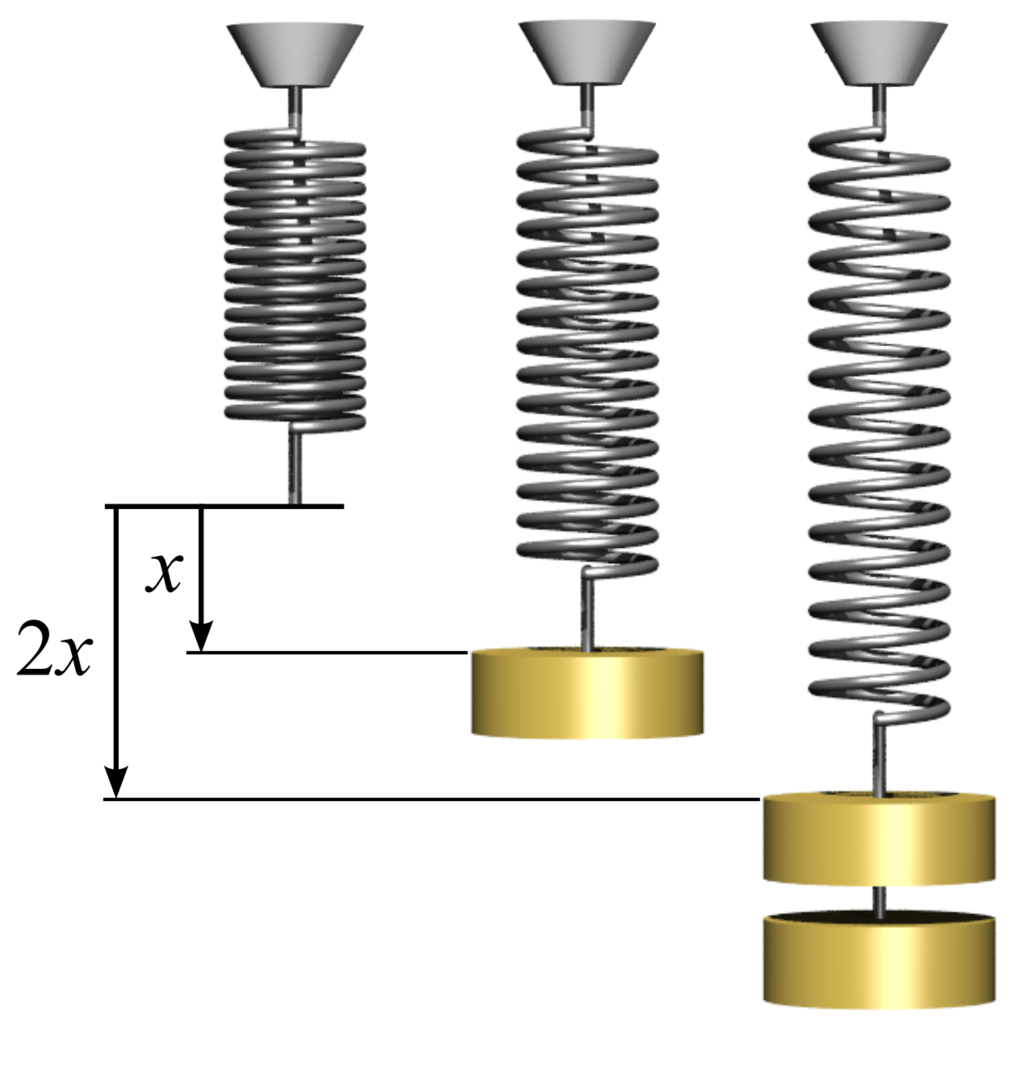
\includegraphics[width=0.3\linewidth]{figures/Hookes-law-springs}
\caption{Hooke's law of spring}
\label{fig:Hookes-law-springs}
\end{figure}

Hooke's law is only a \textbf{first-order linear approximation} to the real response of springs and other elastic bodies to applied forces. It must eventually fail once the forces exceed some limit, since no material can be compressed beyond a certain minimum size, or stretched beyond a maximum size, without some permanent deformation or change of state. Many materials will noticeably deviate from Hooke's law well before those \textbf{elastic limits} are reached.

On the other hand, Hooke's law is an accurate approximation for most solid bodies, as long as the forces and deformations are small enough. For this reason, Hooke's law is extensively used in all branches of science and engineering, and is the foundation of many disciplines such as seismology, molecular mechanics and acoustics. It is also the fundamental principle behind the spring scale, the manometer, and the balance wheel of the mechanical clock.

The modern theory of elasticity generalizes Hooke's law to say that the \textbf{strain (deformation)} of an elastic object or material is proportional to the \textbf{stress} applied to it. However, since general stresses and strains may have multiple independent components, the "proportionality factor" may no longer be just a single real number, but rather a linear map (a tensor) that can be represented by a matrix of real numbers.

In this general form, Hooke's law makes it possible to deduce the relation between strain and stress for complex objects in terms of intrinsic properties of the materials it is made of. For example, one can deduce that a homogeneous rod with uniform cross section will behave like a simple spring when stretched, with a stiffness k directly proportional to its cross-section area and inversely proportional to its length.

\section{Stiffness Tensor for continuous media}
The stresses and strains of the material inside a continuous elastic material (such as a block of rubber, the wall of a boiler, or a steel bar) are connected by a linear relationship that is mathematically similar to Hooke's spring law, and is often referred to by that name.

However, the strain state in a solid medium around some point cannot be described by a single vector. The same parcel of material, no matter how small, can be compressed, stretched, and sheared at the time, along different directions. Likewise, the stresses in that parcel can be at once pushing, pulling and shearing.

In order to capture this complexity, the relevant state of the medium around a point must be represented by two second-order tensors, the \textbf{strain tensor} $ \varepsilon $ (in lieu of the displacement $ X $) and the \textbf{stress tensor} $ \sigma $ (replacing the restoring force $ F $). The analogous of Hooke's spring law for continuous media is then

\begin{equation}
\mathbf{\sigma} = -\mathbf{C} \mathbf{\varepsilon}
\end{equation}

The symmetry of the \textbf{Cauchy stress tensor} $ (\sigma_{ij} = \sigma_{ji}) $ and the generalized Hooke's laws:

\begin{equation}
\sigma_{ij} = c_{ijkl} \varepsilon_kl
\end{equation}

implies that $ c_{ijkl} = c_{jikl} $. Similarly, the symmetry of the \textbf{infinitesimal strain tensor} implies that $ c_{ijkl} = c_{ijlk} $. These symmetries are called the \textbf{minor symmetries} of the \textbf{stiffness tensor} $ (\mathbf{C}) $. This reduces the number of elastic constants from 81 to 36.

If in addition, since the displacement gradient and the Cauchy stress are work conjugate, the stress-strain relation can be deprived from a strain energy density function $ (U) $, then

\begin{equation}
\sigma_{ij} = \dfrac{\partial U}{\partial \varepsilon_{ij}} \Longrightarrow c_{ijkl} = \dfrac{\partial^2 U}{\partial \varepsilon_{ij} \partial \varepsilon_{kl} }
\end{equation}

The arbitrariness of the order of differentiation implies that $ c_{ijkl} = c_{klij} $. These are called the \textbf{major symmetries} of the stiffness tensor. This reduces the number of elastic constants to 21 from 36. The major and minor symmetries indicate that the stiffness tensor has only 21 independent components.

where $ \mathbf{C} $ is a forth-order tensor (that is, a linear map between second-order tensors) called the \textbf{stiffness tensor} or \textbf{elasticity tensor}. One may also write as

\begin{equation}
\mathbf{\varepsilon} = -\mathbf{S} \mathbf{\sigma}
\end{equation}

where the tensor $ \mathbf{S} $, called the compliance tensor, represents the inverse of said linear map.

In a Cartesian coordinate system, the stress and strain tensors can be represented by $ 3 \times 3 $ matrices
\begin{equation}
\mathbf{\varepsilon} = \begin{bmatrix}
\varepsilon_{11} & \varepsilon_{12} & \varepsilon_{13} \\
\varepsilon_{21} & \varepsilon_{22} & \varepsilon_{23} \\
\varepsilon_{31} & \varepsilon_{32} & \varepsilon_{33}
\end{bmatrix}~~~~~ \mathbf{\sigma} = \begin{bmatrix}
\sigma_{11} & \sigma_{12} & \sigma_{13} \\
\sigma_{21} & \sigma_{22} & \sigma_{23} \\
\sigma_{31} & \sigma_{32} & \sigma_{33}
\end{bmatrix}
\end{equation}

Being a linear mapping between the nine numbers $ \sigma_{ij} $ and the nine numbers $ \varepsilon_{kl} $, the stiffness tensor $ \mathbf{C} $ is represented by a matrix of $ 3 \times 3 \times 3 \times 3 = 81 $ real numbers $ C_{ijkl} $. Hooke's law then says that

\begin{equation}
\sigma_{ij} = -\sum_{k=1}^{3} \sum_{l=1}^{3} C_{ijkl} \varepsilon_{kl}
\end{equation}

where $ i $ and $ j $ are 1, 2, or 3.

All three tensors generally vary from point to point inside the medium, and may vary with time as well. The strain tensor $ \mathbf{\epsilon} $  merely specifies the displacement of the medium particles in the neighborhood of the point, while the stress tensor $ \mathbf{\sigma} $  specifies the forces that neighboring parcels of the medium are exerting on each other. Therefore, they are independent of the composition and physical state of the material. The stiffness tensor $ \mathbf{C} $ , on the other hand, is a property of the material, and often depends on physical state variables such as temperature, pressure, and microstructure.

Due to the inherent symmetries of $ \mathbf{\sigma} $, $ \mathbf{\epsilon} $ , and $ \mathbf{C} $ , only 21 elastic coefficients of the latter are independent. For isotropic media (which have the same physical properties in any direction), $ \mathbf{C} $ can be reduced to only two independent numbers, the bulk modulus $ K $ and the shear modulus $ G $ , that quantify the material's resistance to changes in volume and to shearing deformations, respectively.

\section{Principal stresses}
The majority of material strength data is based on uniaxial tensile test results. Usually, allthat you have to work with is the yield strength $ S_y $ and/or the ultimate tensile strength $ S_u $. \\

This is fine if you only have the one normal stress component present: this is true for simple tension or compression members and for parts loaded only in bending.

\begin{figure}[h!]
	\centering
	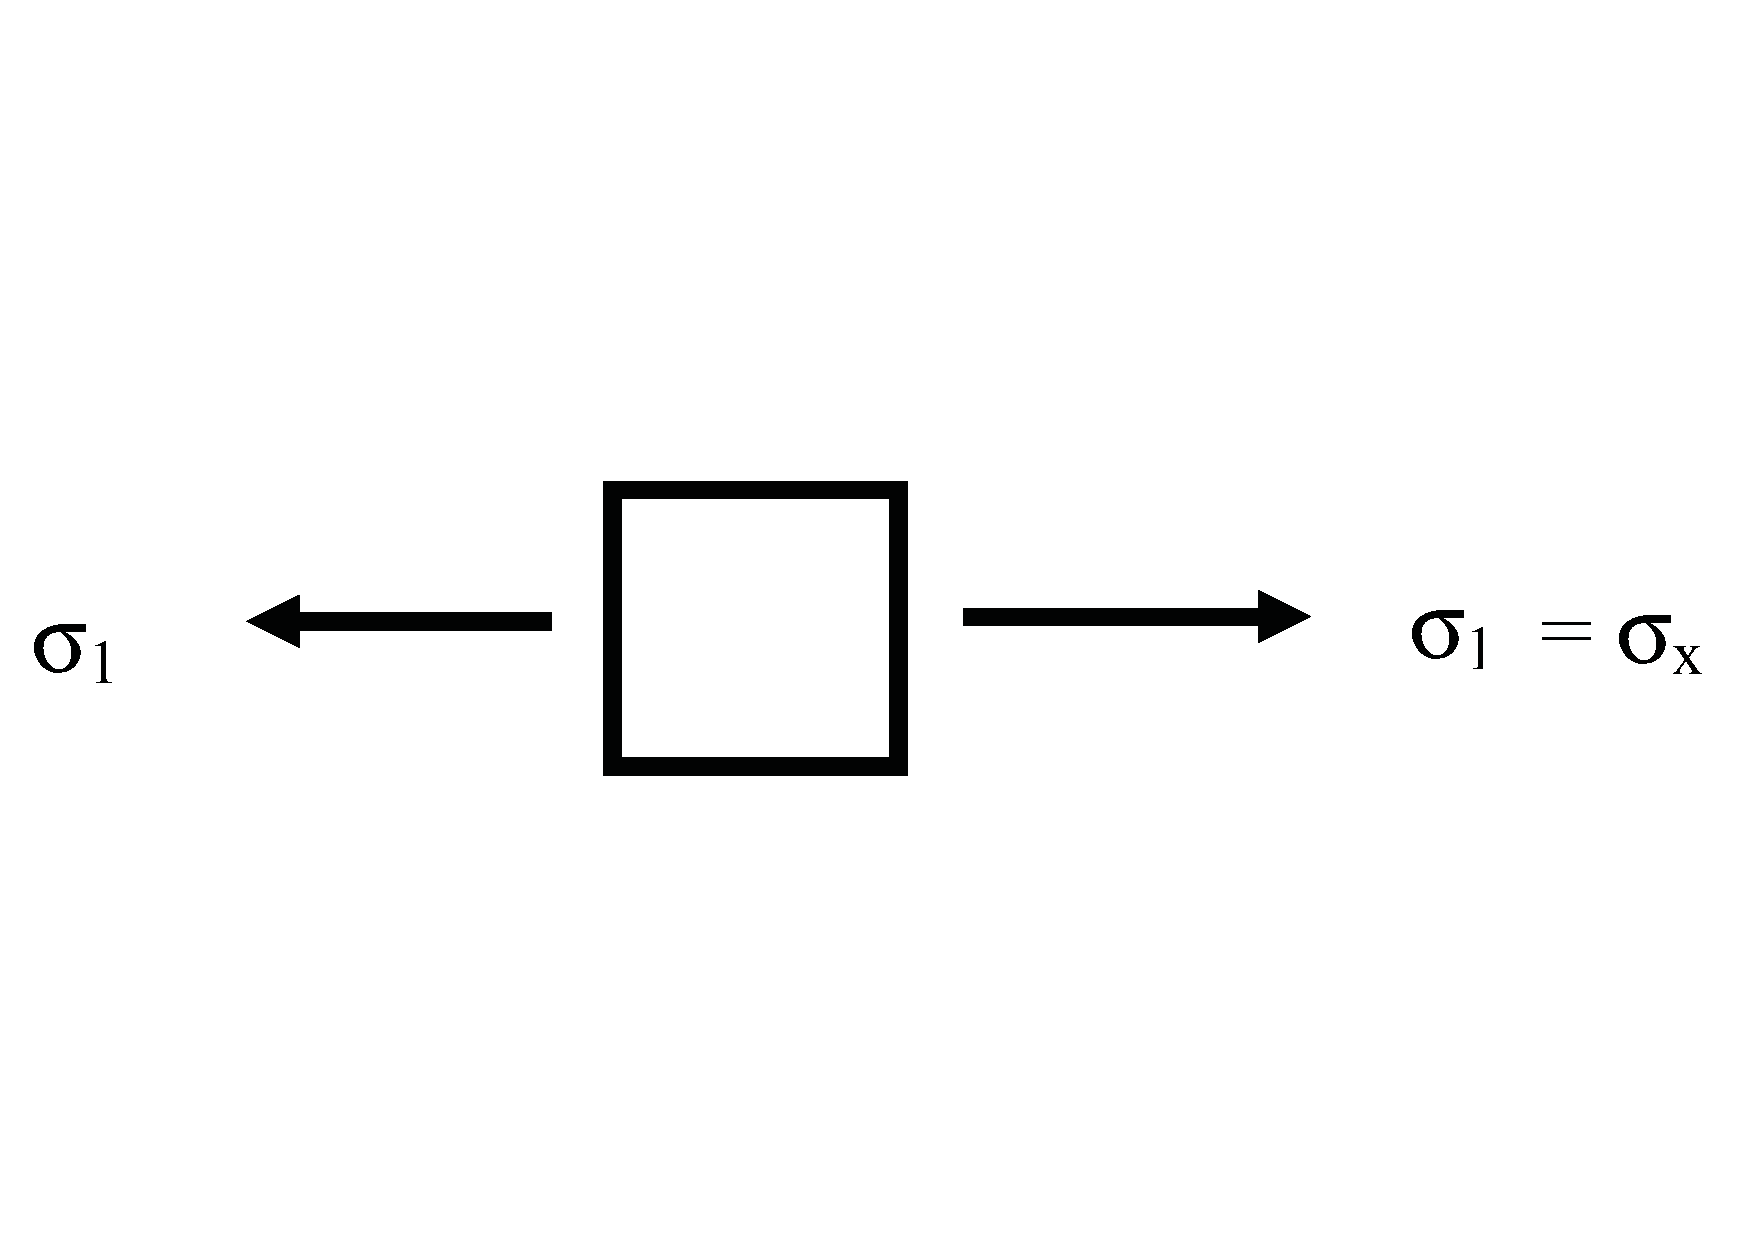
\includegraphics[width=0.3\linewidth]{figures/uniaxial_stress}
	\caption{uniaxial stress}
	\label{fig:uniaxialstress}
\end{figure}

In this case, failure (defined as the onset of plastic deformation) occurs when

\begin{equation}
\sigma_x = \sigma_1 = \frac{S_y}{n}
\end{equation}

$ n $ is the factor of safety.

In many loading cases, we have more than just one normal stress component.E.g. in torsion, we have a single shear stress component:

\begin{figure}[h!]
\centering
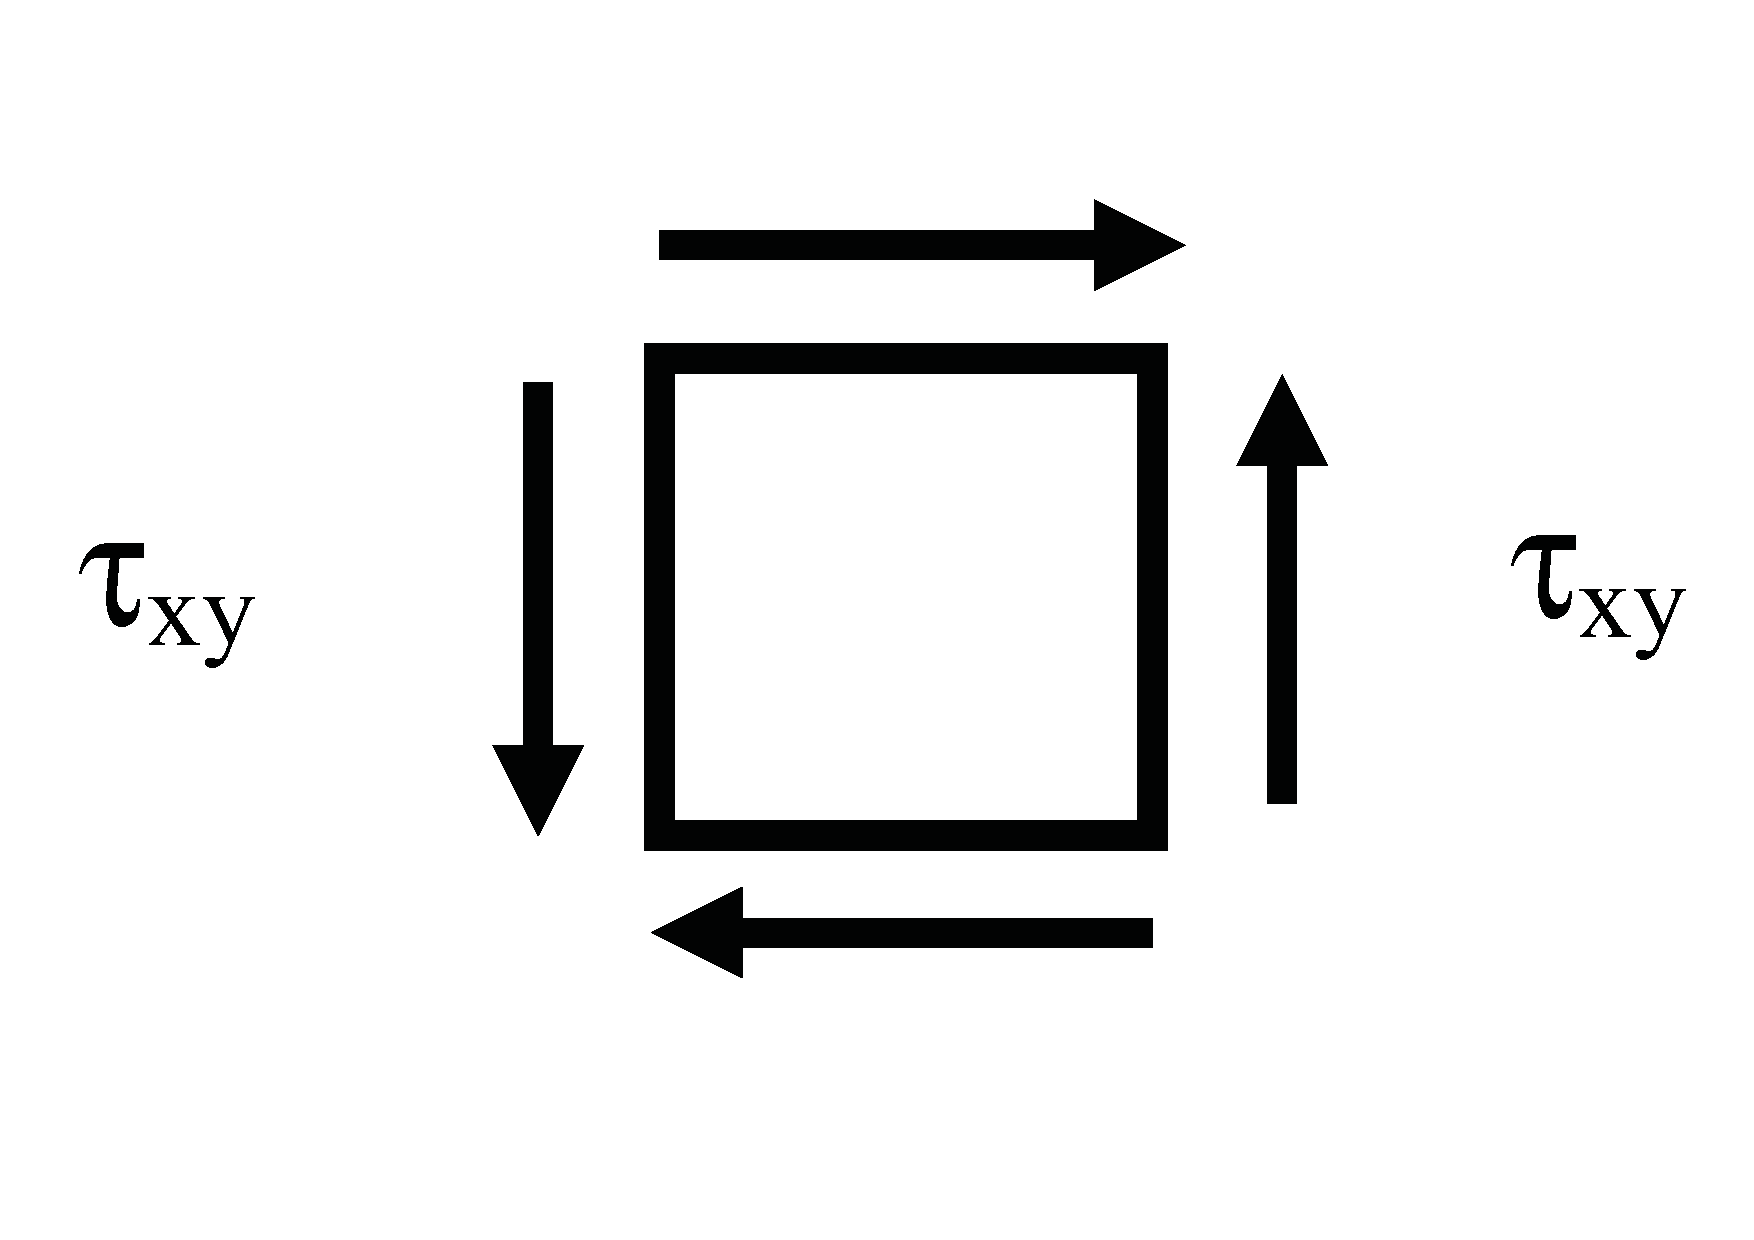
\includegraphics[width=0.3\linewidth]{figures/shear_stress}
\caption{shear stress}
\label{fig:shearstress}
\end{figure}

Or, combined bending and torsion in a shaft:

\begin{figure}[h!]
\centering
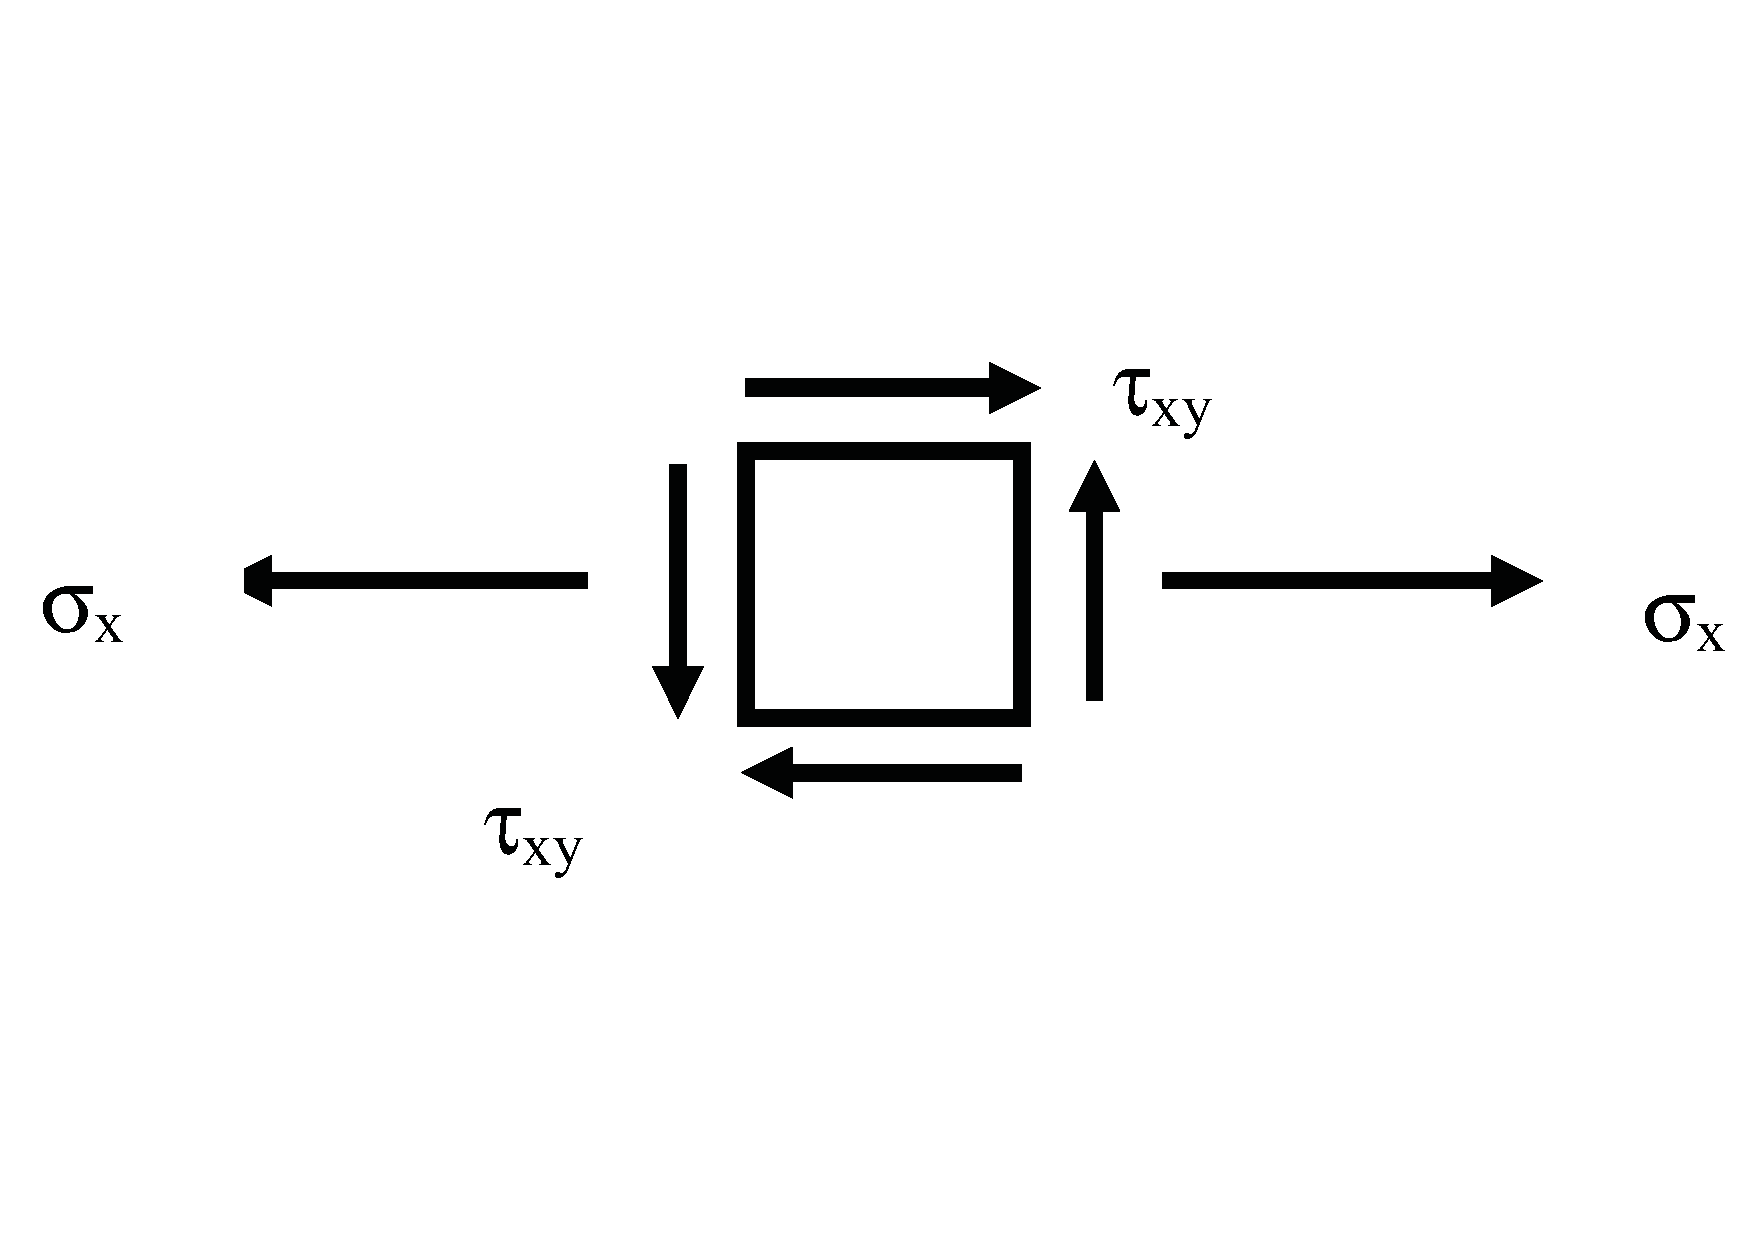
\includegraphics[width=0.3\linewidth]{figures/combined_stress}
\caption{combined stress}
\label{fig:combinedstress}
\end{figure}

These cases can all be reduced to a simple biaxial case by finding the principal stresses, $ \sigma_1 $ and $ \sigma_2 $:

\begin{figure}[h!]
\centering
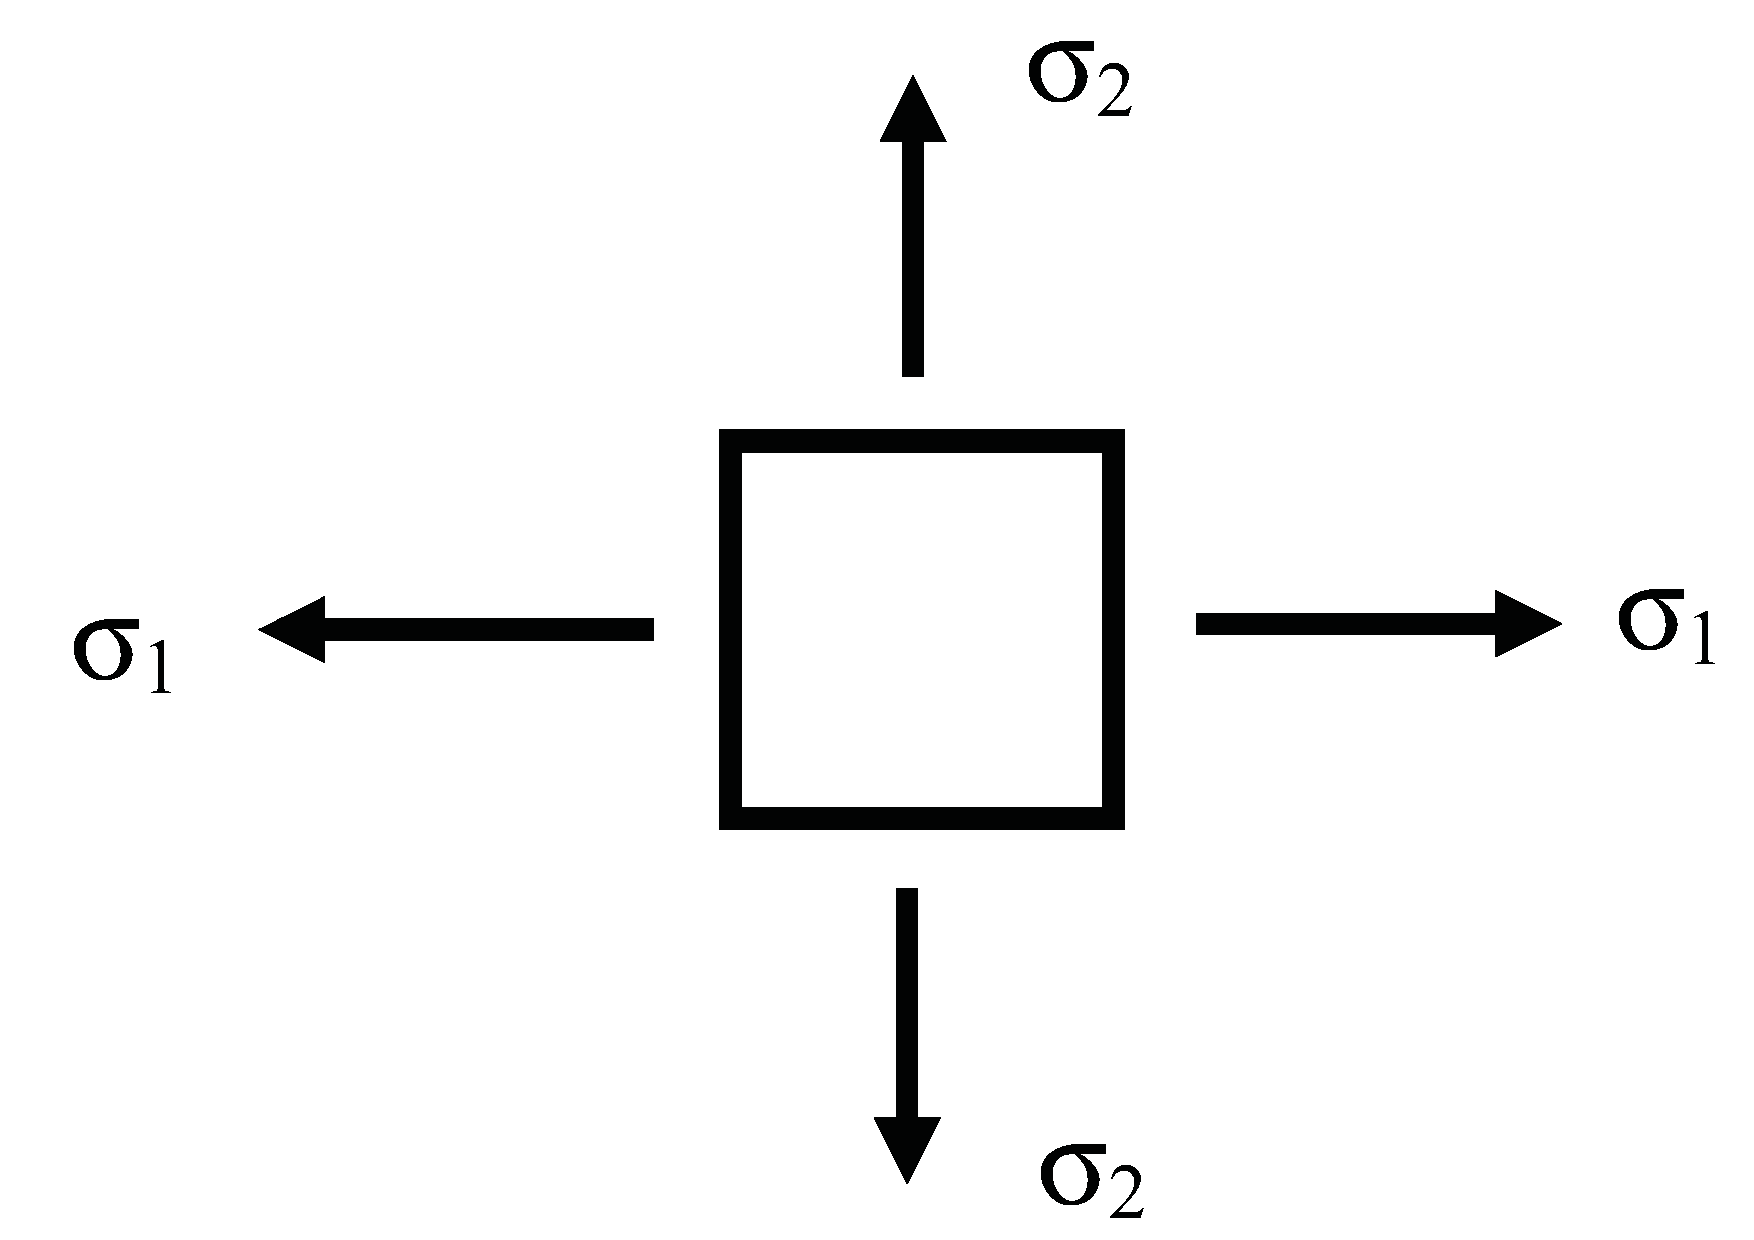
\includegraphics[width=0.3\linewidth]{figures/principal_stress}
\caption{principal stress}
\label{fig:principalstress}
\end{figure}

\section{Mises stress}

\begin{equation}\label{key}
\sigma_v^2 = \dfrac{ \left( \sigma_{11}-\sigma_{22} \right)^2 + \left( \sigma_{22}-\sigma_{33} \right)^2 + \left( \sigma_{33}-\sigma_{11} \right)^2 + 6 \left( \sigma_{23}^2 + \sigma_{31}^2 + \sigma_{12}^2 \right)}{2}
\end{equation}